\section{Projektmanagement}

\subsection{Projektübersicht}
Das Hauptziel dieser Bachelorarbeit ist die Analyse, Absicherung und Abstrahierung eines krisenresistenten Software Defined Netzwerkes.

\subsubsection{Ziele der Projektes}
Die Bachelorarbeit wurde in drei Teile gegliedert:
\begin{itemize}
	\item Phase 1: Analyse
	\begin{itemize}
		\item Sämtliche Analyse der SD-A Lösung und Identifizierung der kritischen Elemente der Verfügbarkeit (LISP Database, Radius, SGT Access-list,…) und der Network Services (NTP, DNS, Lizenzen, ….)
	\end{itemize}
	\item Phase 2: Absicherung
	\begin{itemize}
		\item Erstellung von Technische Design und Ansätze um die SD-A Lösung Krisenresistenter zu machen.
	\end{itemize}
	\item Phase 3: Abstrahierung
	\begin{itemize}
		\item Entwicklung eines Operations Orchestrators für 2-3 Use Cases.
	\end{itemize}
	
\end{itemize}

\subsection{Projektorganisation}
Diese Bachelorarbeit wird von zwei Personen umgesetzt und durch zwei Betreuer überwacht.

\subsubsection{Organisationsstruktur}
\begin{figure}[H]
	\centering
	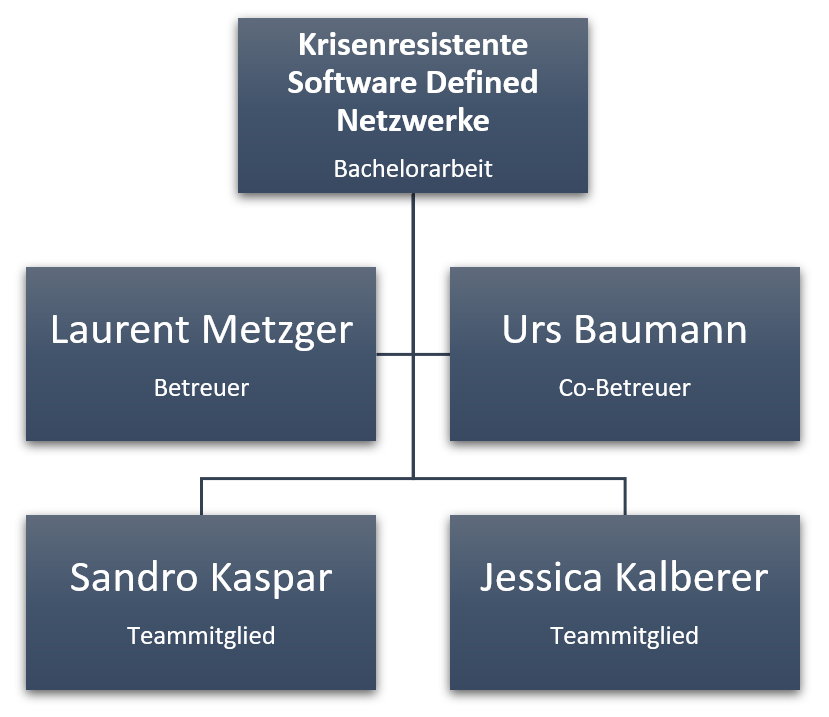
\includegraphics[width=0.7\linewidth]{img/Projektplanung/Organisationsstruktur}
	\caption{Organisationsstruktur}
	\label{fig:Organisationsstruktur}
\end{figure}


\subsection{Management Abläufe}
Für die Umsetzung der Bachelorarbeit stehen insgesamt 14 Wochen und pro Person 360 Stunden zur Verfügung. In einer Woche liegt das Arbeitspensum von knapp 26 Stunden pro Person vor. Das Projekt startet am 17. September 2018 und endet am 21. Dezember 2018.

\subsubsection{Zeitliche Planung}
Die zeitliche Planung, sowie die Verwaltung der Arbeitspakete erfolgte auf Waffle.io. Die Planung wird während dem Projekt laufend aktualisiert und angepasst. Die Arbeitszeiten werden während der Arbeitsausführung mit Toggle erfasst.

\begin{figure}[H]
	\centering
	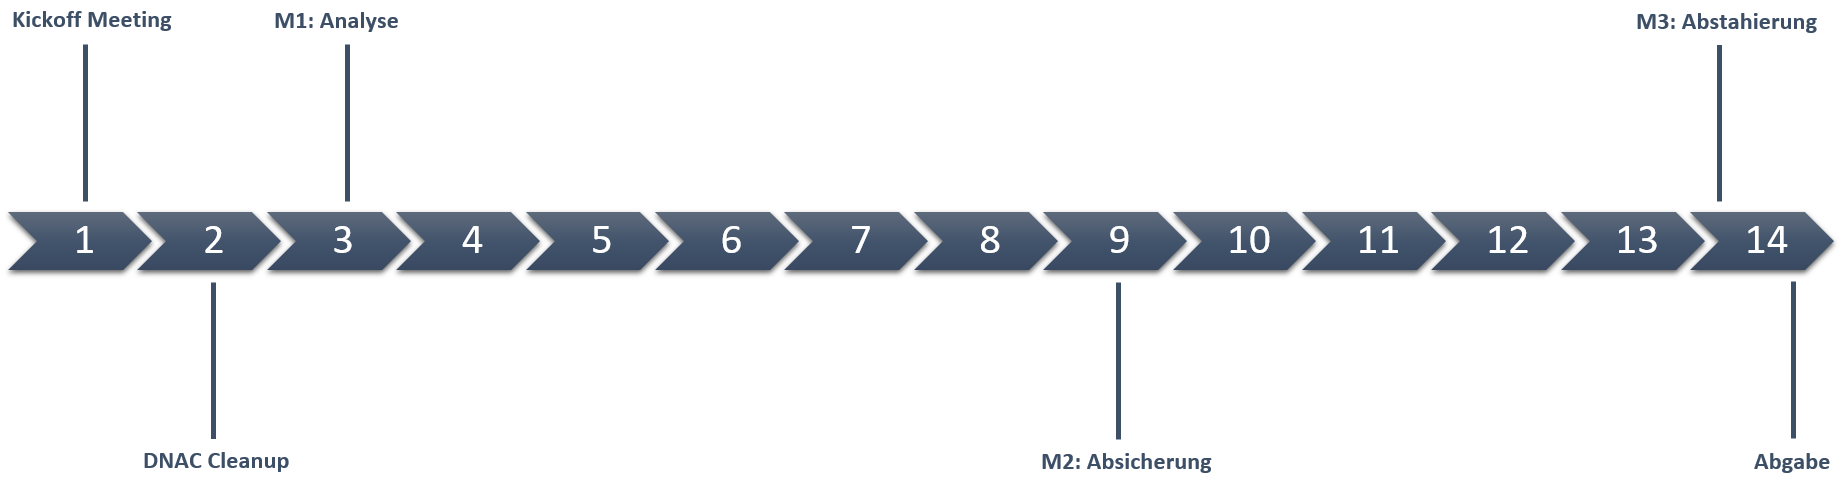
\includegraphics[width=1\linewidth]{img/Projektplanung/Projektplanung_v1}
	\caption{Projektplanung}
	\label{fig:Projektplanung}
\end{figure} 


\subsubsection{Meilensteine}
Folgende Meilensteine sind für das Projekt definiert:
\begin{table}[H]
	\rowcolors{2}{gray!25}{white}
	\centering
	\begin{tabularx}{\textwidth}{p{1cm}| p{2.5cm}| X}
		\rowcolor{gray!50}
		\textbf{Nr} & \textbf{Datum} & \textbf{Meilenstein} \\
		\hline	
		 & 18.09.2018 & Kickoff Meeting \\
		M0 & 30.09.2018 & DNAC Cleanup \\
		M1 & 07.10.2018 & Analyse \\
		M2 & 18.11.2018 & Absicherung \\
		M3 & 20.12.2018 & Abstrahierung \\
		 & 21.12.2018 & Abgabe \\
	\end{tabularx}
	\caption{Meilensteine}
	\label{tab:Meilensteine}
\end{table}



\subsubsection{Arbeitspakete}
Alle Arbeitspakete werden in Waffle.io erfasst und sind unter folgendem Link ersichtlich:
\href{Waffle.io}{https://waffle.io/night28/HSR\_BA}
\subsubsection{Besprechungen}
Die Besprechungen mit dem Betreuer finden an den nachfolgend aufgelisteten Tagen statt:
\begin{itemize}
	\item jeden Mittwoch zwischen 10.30 - 11.30 Uhr
\end{itemize}

Offene Traktanden und Probleme werden mit dem Betreuer diskutiert. Nach dieser Besprechung wird jeweils in einem Team-Meeting das weitere Vorgehen geplant.


\subsection{Infrastruktur}
Die Organisation der Arbeit und Teammitglieder wird durch folgende Werkzeuge unterstützt:

\begin{figure}[H]
	\centering
	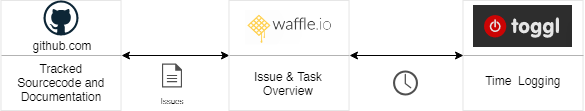
\includegraphics[width=13cm]{img/EingesetzteToolsZurOrganisation.png}
	\caption{Übersicht über die Verknüpfung der eingesetzten Werkzeuge zur internen Organisation.}
	\label{fig:Interne Organisationsstruktur}
\end{figure} 

Unsere Tools sind unter folgenden Links einsehbar:
\paragraph{GitHub} \href{https://github.com/night28/HSR\_BA}{https://github.com/night28/HSR\_BA} 

\paragraph{Waffle.io} \href{https://waffle.io/night28/HSR\_BA}{https://waffle.io/night28/HSR\_BA}

\paragraph{Toggl} \href{https://toggl.com/}{https://toggl.com/}
 
\subsection{Risiko Management}

\subsubsection{Umgang mit Risiken}
Risiken lassen sich leider nicht immer vermeiden. Aus diesem Grund sind nachfolgend mögliche Risiken aufgeführt. Erfahrungen aus der Studienarbeit sind wesentlich in die Gewichtung der einzelnen Risiken eingeflossen. Des Weiteren wurden vorbeugende Massnahmen definiert, um die Eintrittswahrscheinlichkeit von Risiken mit schwerwiegenden Konsequenzen zu reduzieren. Für den Fall, dass ein Risiko dennoch eintreten sollte, sind entsprechende Massnahmen definiert um den Schaden möglichst gering zu halten.
Sollten sich während dem Projekt neue potenzielle Risiken zeigen, wird dieses Dokument laufend aktualisiert.

\begin{landscape}
\subsubsection{Risiken}
\newcommand*\rot{\rotatebox{90}}
\begin{longtable}{|m{0.5cm}|m{3cm}|m{5cm}|m{0.75cm}|m{0.75cm}|m{0.75cm}|m{5cm}|m{5cm}|} 
	\hline
	\rot{Nummer} & \rot{Titel} & \rot{Beschreibung} & \rot{\shortstack[l]{maximaler\\Schaden [h]}} & \rot{\shortstack[l]{Eintritts-\\wahrscheinlichkeit}} & \rot{\shortstack[l]{Gewichteter\\Schaden [h]}} & \rot{Vorbeugung} & \rot{\shortstack[l]{Verhalten beim\\Eintreten}} \\
	\hline\hline
	1 & Ausfall eines Teammitglieds & Ausfall auf Grund unvorhergesehener Ereignisse wie Krankheit, Unfall etc. & 40 & 15\% & 6 & Reserven einplanen, Kommunikation sicherstellen, damit andere Teammitglieder die Aufgaben übernehmen können & Tasks des ausgefallen Mitglieds möglichst auf die anderen Teammitglieder aufteilen. \\ 
	\hline
	2 & Hardwareausfall DNA-Center & DNA-Center Appliance fällt durch Hardwaredefekt aus & 50 & 5\% & 2.5 & keine Verbeugenden Massnahmen möglich & Austausch im Rahmen der Garantie veranlassen \\
	\hline
	3 & Fehlendes Know-How & Da viele der Themen neu sind, kann entsprechendes Wissen fehlen & 40 & 10\% & 4 & Zeit einplanen um sich in neue Themen einzuarbeiten & Fehlendes Wissen sobald wie möglich aneignen. Bei Bedarf Rat der Betreuer einholen \\
	\hline
	4 & Konflikte im Team & Das Team ist sich bezüglich wichtigen Entscheidungen uneinig & 25 & 10\% & 2.5 & Entscheidungen stets mit Begründung dokumentieren & Kann auch mit Hilfe der Doku keine Einigung gefunden werden, fachnlichen Rat des Betreuers einholen \\
	\hline
	5 & Missverständnisse im Team & Im Team herscht Uneinigkeit über bereits getroffene Entscheidungen & 30 & 20\% & 6 & Protokolle führen und Entscheidungen klar dokumentieren & Protokolle und Dokumentationen beiziehen \\
	\hline
	6 & Ausfall Server / Netzwerkinfrastruktur & Ausfall der von der HSR zur Verfügung gestellten Infrastrukturkomponenten & 30 & 5\% & 1.5 & Keine Vorbeugenden Massnahmen möglich & Sobald die Infrastruktur wieder verfügbar ist, Systeme erneut in Betrieb nehmen \\
	\hline
	7 & Lieferverzögerung Hardware & Die von Cisco bestellte Hardware kommt später als angekündigt & 40 & 20\% & 8 & Keine Vorbeugenden Massnahmen möglich & Projektplanung an neue Gegebenheiten anpassen, notfalls Projektumfang in Absprache mit Betreuer anpassen \\
	\hline
	8 & Zeitaufwände falsch geschätzt & Auf Grund falscher Schätzungen kommt es zu Verzögerungen im Projekt & 30 & 20\% & 6 & Laufende Kontrolle des Projektfortschritts um Probleme frühzeitig zu erkennen, Reserven einplanen & Verbleibende Schätzungen korrigieren, Planung anpassen \\
	\hline
	9 & Datenverlust & Verlust von projektbezogenen Daten wie Dokumentationen, Konfigurationen etc. & 40 & 5\% & 2 & Regelmässige und verteilte Backups aller Daten erstellen & Verlorenen Daten aus Backups wiederherstellen, fehlende Daten neu erarbeiten \\
	\hline
	10 & Unausgereifte Software & Verzögerung des Projektes durch unvorhergesehene Hürden, da Software nicht genügend auf Funktionalität getestet und Dokumentiert. Software steht noch in einem frühen Release. & 80 & 10\% & 8 & Über aktuelle Funktionalitäten und Bugs informieren & Bugs reporten und bei Möglichkeit diese umgehen. Falls nötig Hilfe beim Hersteller suchen. \\
	\hline
\end{longtable}

\end{landscape}

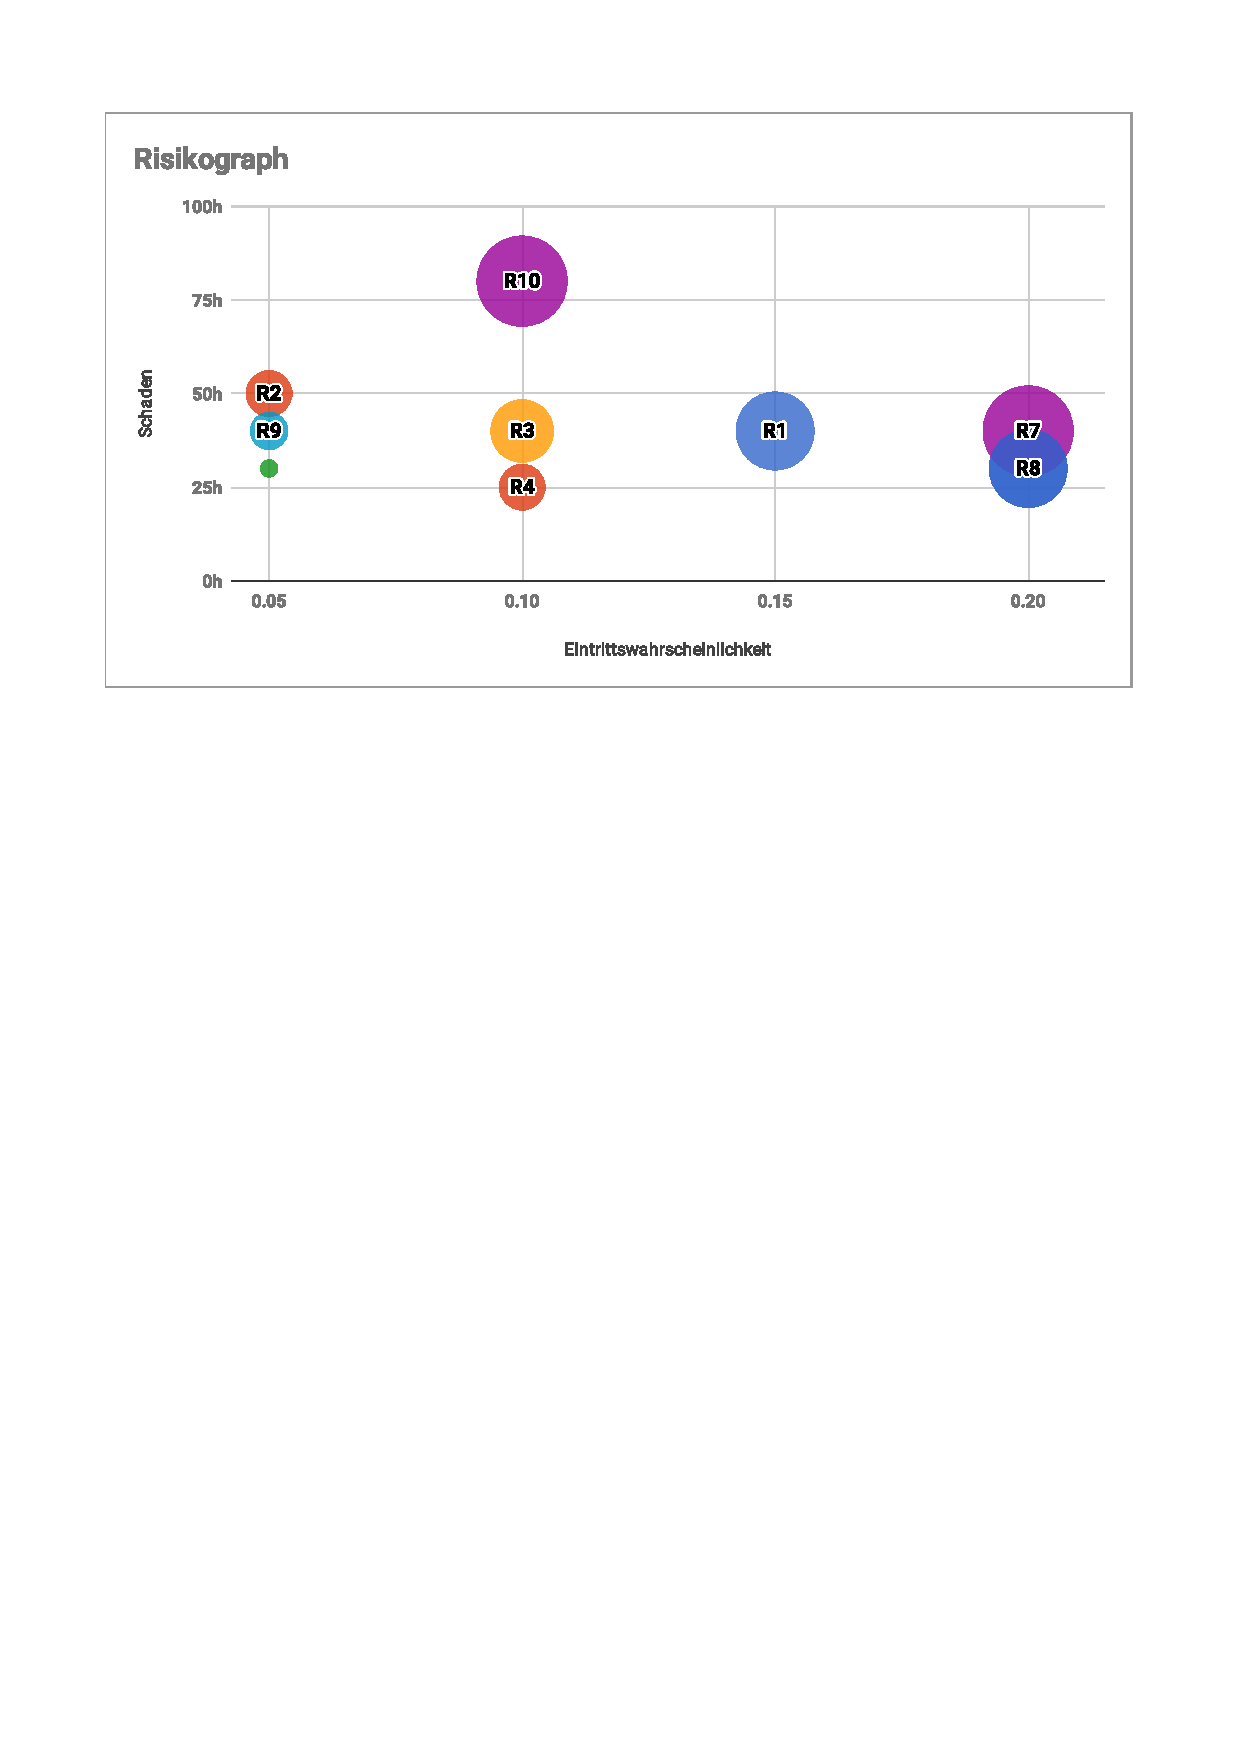
\includepdf{pdfincludes/risikograph}

\subsubsection{Eingetretene Risiken}

\paragraph{Lieferverzögerung Hardware} 
Der Liefertermin für den ENCS 5400 wurde auf Mitte November angekündigt und sollte aber noch beschleunigt werden. Die tatsächliche Lieferung erfolge schliesslich am 21. November 2018. Durch diese Veränderung und auch weil die Umsetzung der Absicherung mehr Aufwand in Anspruch nahm, musste der Meilenstein der Phase Absicherung nach hinten geschoben werden. Durch den Einsatz des ENCS 5400 wurden des Weiteren noch Anpassungen an der Architektur nötig, was einen erhöhten Aufwand der Phase Umsetzung zur Folge hatte. Zusätzlich wurde entschieden, dass die Abstrahierung parallel zur Absicherung schon gestartet wird und somit keine explizite Trennung der beiden Phasen mehr nötig ist.

\paragraph{Unausgereifte Software} 
Das DNA Center befand sich zu Beginn der Studienarbeit in der Version 1.1.6 und wurde während der Bachelorarbeit anschliessend von Anfang an mit der Version 1.2.5 eingesetzt. In einigen Aspekten merkt man, dass das DNA Center sich noch im Aufbau befindet und noch diverse Bugs besitzt. Es wurden jedoch viele Bugs die in der Studienarbeit auftraten behoben, was vor allem den Aufwand beim Provision mittels PnP enorm vereinfacht hat. In der Bachelorarbeit neu aufgetretene Bugs wurden unter dem Kapitel \ref{Feature Requests und Bugs} Feature Requests und Bugs erfasst. Es ist vor allem zu erwähnen, dass der ENCS5400 im DNA Center verwaltet wird und somit auch der ISRv und weitere virtuelle Devices komplett über das DNA Center deployed werden. Dies führte in einigen Fällen beim Deploy der Devices zu nicht nachvollziehbaren Problemen. Nachfolgend eine Übersicht über die Releases des DNA Centers.

\begin{table}[H]
	\rowcolors{2}{gray!25}{white}
	\centering
	\begin{tabularx}{\textwidth}{X | l}
		Cisco Digital Network Architecture Center, Release 1.1.2      & 26.01.2018        \\
		\hline
		Cisco Digital Network Architecture Center, Release 1.1.3      & 08.03.2018        \\
		\hline
		Cisco Digital Network Architecture Center, Release 1.1.4      & 03.04.2018        \\
		\hline
		Cisco Digital Network Architecture Center, Release 1.1.5      & 06.04.2018        \\
		\hline
		\textbf{Cisco Digital Network Architecture Center, Release 1.1.6}      & \textbf{17.05.2018}        \\
		\hline
		Cisco Digital Network Architecture Center, Release 1.1.7      & 09.06.2018        \\
		\hline
		Cisco Digital Network Architecture Center, Release 1.1.8      & 19.07.2018        \\
		\hline
		Cisco Digital Network Architecture Center, Release 1.2        & 05.06.2018        \\
		\hline
		Cisco Digital Network Architecture Center, Release 1.2.1      & 15.06.2018        \\
		\hline
		Cisco Digital Network Architecture Center, Release 1.2.2      & 22.06.2018        \\
		\hline
		Cisco Digital Network Architecture Center, Release 1.2.3      & 13.08.2018        \\
		\hline
		Cisco Digital Network Architecture Center, Release 1.2.4      & 06.09.2018        \\
		\hline
		\textbf{Cisco Digital Network Architecture Center, Release 1.2.5}      & \textbf{01.10.2018}        \\
		\hline
		Cisco Digital Network Architecture Center, Release 1.2.6      & 31.10.2018        
	\end{tabularx}
	\caption{Release Notes DNA Center \cite{dnac-releasenotes}}
	\label{tab:Release Notes DNA Center}
\end{table}



